% SIAM Article Template
\documentclass[r]{siamart171218}
% Packages and macros go here
\usepackage[english]{babel}
\usepackage{amsmath}
\usepackage{amssymb}
\usepackage{amsfonts}
\usepackage{array}
\usepackage{graphicx}
\usepackage{epsfig}
\usepackage{float}
\usepackage{fullpage}
\usepackage{color}
\usepackage{enumitem}  
\usepackage{epstopdf}
\usepackage{stmaryrd}

% Title. If the supplement option is on, then "Supplementary Material"
% is automatically inserted before the title.
%\title{On the weak coupling of 3D and 1D second order elliptic problems}
\title{Coupling PDEs on 3D-1D domains with Lagrange multipliers}

% Authors: full names plus addresses.
\author{Miroslav Kuchta, Federica Laurino, Kent-Andre Mardal, Paolo Zunino,\thanks{Authors are listed in alphabetical order}}

\begin{document}

\maketitle

% REQUIRED
\begin{abstract}
These are personal notes written to keep track of the developments on this topic, to be kept confidential.
\end{abstract}

% REQUIRED
\begin{keywords}
elliptic problems, high dimensionality gap, essential coupling conditions, Lagrange multipliers
\end{keywords}

% REQUIRED
\begin{AMS}
n.a.
\end{AMS}

% >>>>>>>>>>>>>>>>>>>>>>>>>>>>>>>>>>>>>>>>>>>>>>>>>>>>>>>>>>>>>>>>>>>>>>>>>>>>>>>>>>>>>>>>>>>>>>>>>>>>
 
% definitions here

\def\ud{u_{\odot}}
\def\udh{u_{\odot, h}}
\def\vd{v_{\odot}}
\def\uf{u_{\ominus}}
\def\up{u_{\oplus}}
\def\eps{\epsilon}
\def\nn{\boldsymbol n}
\def\rr{\boldsymbol r}
\def\RR{\boldsymbol R}
\def\kk{\boldsymbol k}
\def\ss{\boldsymbol s}
\def\uu{\boldsymbol u}
\def\vv{\boldsymbol v}
\def\xx{\boldsymbol x}
\def\bu{\overline{u}}
\def\bv{\overline{v}}
\def\tu{\widetilde{u}}
\def\tv{\widetilde{v}}
\def\TT{\boldsymbol T}
\def\NN{\boldsymbol N}
\def\BB{\boldsymbol B}
\def\ttu{\widetilde{\widetilde{u}}}
\def\ttv{\widetilde{\widetilde{v}}}
\def\cv{\check{v}}
\def\mesh{{\cal T}^h}
\def\ball{{\cal B}}
\def\R{\mathbb{R}}
\def\D{\mathcal{D}}
\def\DD{\partial\mathcal{D}}
\def\trace{\overline{\mathcal{R}}}
\def\ext{\mathcal{E}}
\def\ide{\mathcal{I}}
\def\ii{\hat{\imath}}
\newcommand{\avrd}[1]{\overline{\overline{#1}}}
\newcommand{\avrc}[1]{\overline{#1}}
\newcommand{\refe}[1]{{#1}_{\mathrm{ref}}}
\newcommand{\norm}[1]{\lVert{#1}\rVert}

\newcommand{\vertiii}[1]{{\left\vert\kern-0.25ex\left\vert\kern-0.25ex\left\vert #1 
    \right\vert\kern-0.25ex\right\vert\kern-0.25ex\right\vert}}

\newtheorem{thm}{Theorem}[section]
\newtheorem{prop}{Property}[section]
\theoremstyle{remark}
\newtheorem{remark}{Remark}[section]
 
% >>>>>>>>>>>>>>>>>>>>>>>>>>>>>>>>>>>>>>>>>>>>>>>>>>>>>>>>>>>>>>>>>>>>>>>>>>>>>>>>>>>>>>>>>>>>>>>>>>>>
\section{Introduction}\label{sec:intro}

We address the geometrical configuration of the problem for a 3D coupled problem formulation based on from Dirichlet-Neumann interface conditions. Then, we apply a model reduction technique that transforms the problem into 3D-1D coupled PDEs. We develop and analyze a robust definition of the coupling operators form a 3D domain, $\Omega$, to 1D manifold, $\Lambda$, and vice versa. This is a non trivial objective because the standard trace operator form a domain $\Omega$ to a subset $\Lambda$ is not well posed if $\Lambda$ is a manifold of co-dimension two of $\Omega$.

% >>>>>>>>>>>>>>>>>>>>>>>>>>>>>>>>>>>>>>>>>>>>>>>>>>>>>>>>>>>>>>>>>>>>>>>>>>>>>>>>>>>>>>>>>>>>>>>>>>>>
\section{Problem setting}\label{sec:setting}

Let $\Omega \subset \mathbb{R}^3$ be a bounded, convex open set. Let $\Sigma$ be a generalized cylinder embedded into $\Omega$ and be $\Omega_\oplus = \Omega \setminus \overline{\Sigma}$ be the complementary set of the cylinder. We also introduce the set $\Lambda$, a 1D manifold that is the centerline of $\Sigma$. We define the arc-length coordinate along $\Lambda$, denoted by $s \in (0,S)$. We denote with $\mathcal{D}(s)$ and $\partial\mathcal{D}(s)$ a cross section of $\Sigma$ and its boundary, respectively. In what follows, we assume for simplicity of notation that $\Sigma$ has a constant cross section, but this is not a restriction of the approach. We also assume that $\Sigma$ crosses $\Omega$ from side to side and we call $\Gamma$ the lateral (cylindrical) surface of $\Sigma$, while the upper and lower side faces of $\Sigma$ belong to $\partial\Omega$. We refer to Figure \ref{fig1} for an illustration of the notation. 

\begin{figure}
\begin{center}
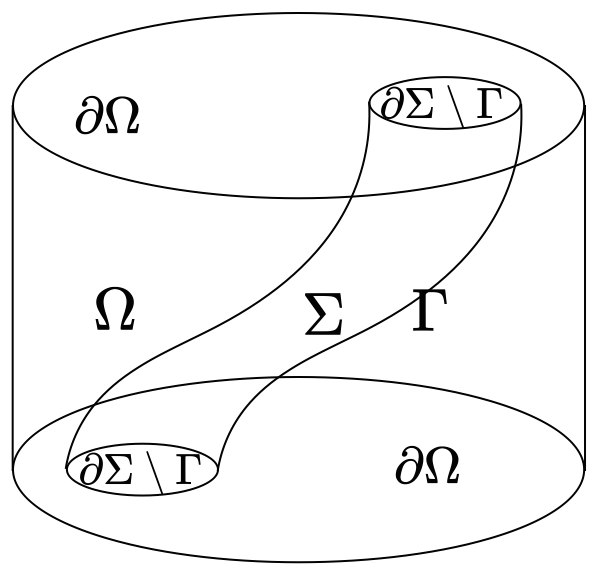
\includegraphics[width=0.5\textwidth]{3D-1D-simple.png}
\end{center}
\caption{Geometrical setting of the problem}
\label{fig1}
\end{figure}

We consider the problem arising from \emph{Dirichlet-Neumann} conditions. 
It consists to find $\up,\uf$ s.t.:
\begin{subequations}\label{eq:dirneu}
\begin{align}
\label{eq:dirneu1}
- \Delta \up  + \up &= f  && \text{ in } \Omega_{\oplus},\\
\label{eq:dirneu2}
- \Delta \uf  + \uf &= g  && \text{ in } \Sigma,\\
\label{eq:dirneu3}
-\nabla \uf \cdot \nn_{\ominus} &= -\nabla \up \cdot \nn_{\ominus}  && \text{ on } \Gamma,\\
\label{eq:dirneu4}
\uf &= \up && \text{ on }  \Gamma,\\
\label{eq:dirneu5}
\up &= 0 && \text{ on } \partial \Omega\,.
\end{align}
\end{subequations}

The objective of this work is to derive and alalyze a simplified version of problem \eqref{eq:dirneu}, where the domain $\Sigma$ shrinks to its centerline $\Lambda$ and the corresponding partial differential equation is averaged on the cylinder cross section, namely $\mathcal{D}$. This new problem setting will be called the \emph{reduced} problem. Form the mathematical standpoint it is more challenging than \eqref{eq:dirneu}, because it involves the coupling of 3D/1D elliptic problems.
For the model reduction process, we decompose integrals as follows, for any sufficiently regular function $w$,
\begin{equation*}
\int_\Sigma w d\omega 
= \int_\Lambda \int_{\mathcal{D}} w d\sigma ds
= \int_\Lambda |\mathcal{D}|\avrd{w} ds\,,
\quad
\int_{\Gamma} w d\sigma 
= \int_\Lambda \int_{\partial\mathcal{D}} w d\gamma ds
= \int_\Lambda  |\partial \mathcal{D}| \avrc{w} ds\,,
\end{equation*}
where $\avrd{w}, \ \avrc{w}$ denote the following mean values respectively,
\begin{equation*}
\avrd{w} = |\mathcal{D}|^{-1} \int_{\mathcal{D}} w d\sigma\,,
\quad
\avrc{w} = |\partial\mathcal{D}|^{-1} \int_{\partial\mathcal{D}} w d\gamma\,.
\end{equation*}

We apply the model reduction approach at the level of the variational formulation.
We start from the variational formulation of problem \eqref{eq:dirneu}, 
that is to find $\up \in H^1_{\partial\Omega}(\Omega_\oplus), \ \uf \in H^1_{\partial\Sigma\setminus\Gamma}(\Sigma), \ \lambda \in H^{-\frac12}(\partial\Sigma)$ s.t.
\begin{subequations}\label{eq:weak_dirneu}
\begin{align}
&(u_\oplus,v_\oplus)_{H^1(\Omega_\oplus)} + (u_\ominus,v_\ominus)_{H^1(\Sigma)} 
+ \langle v_\ominus - v_\oplus, \lambda \rangle_{H^{-\frac12}(\Gamma)} 
\\
\nonumber
&\qquad\qquad = (f,v_\oplus)_{L^2(\Omega_\oplus)} + (g,v_\ominus)_{L^2(\Sigma)}
\quad \forall v_\oplus \in H^1_{\partial\Omega}(\Omega_\oplus), \ v_\ominus \in H^1_{\partial\Sigma\setminus\Gamma}(\Sigma)
\\
& \langle u_\ominus - u_\oplus, \mu \rangle_{H^{-\frac12}(\Gamma)} = 0
\quad \forall  \mu \in H^{-\frac12}(\Gamma)\,,
\end{align}
\end{subequations}
where $\langle v, \mu \rangle_{H^{-\frac12}(\Gamma)}$ denotes the duality pairing between 
$ \mu \in H^{-\frac12}(\Gamma)$ and $v \in H^{\frac12}(\Gamma)$.
In this case, the additional variable $\lambda$ is equivalent to $\lambda  = - \nabla \uf \cdot \nn_\ominus$.

Using the averaging tools for the model reduction approach, we end up with a reduced problem
for the unknown $u$ defined on the entire 3D domain $\Omega$, coupled with the unknown $\ud$, defined on the 1D manifold $\Lambda$
and a Lagrange multiplier $L$ defined on $\Lambda$. In the reduced problem the multiplier assumes the following interpretation,
\begin{equation*}
L = - \frac{1}{|\partial{\cal D}|} \int_{\partial{\cal D}} \nabla \uf \cdot \nn_\ominus
   = - \frac{1}{|\partial{\cal D}|} \int_{\partial{\cal D}} \lambda \,.
\end{equation*}

We consider two alternative formulations. The scope of this work is to compare them, 
with the aim to determine which is the most suitable as a computational model based on 3D-1D coupled PDEs.

% >>>>>>>>>>>>>>>>>>>>>>>>>>>>>>>>>>>>>>>>>>>>>>>>>>>>>>>>>>>>>>>>>>>>>>>>>>>>>>>>>>>>>>>>>>>>>>>>>>>>
\subsection{Problem 1}
The idea is to couple a 3D PDE with a 1D one, using a Lagrange multiplier space defined on a 2D surface that surrounds the 1D manifold.
Let $\langle \cdot , \cdot \rangle_\Gamma$ denote the duality pairing between 
$H^\frac12_{00}(\Gamma)$ and $H^{-\frac12}(\Gamma)$.
The problem consists to find $u \in H^1_0(\Omega),\ \ud \in H^1_0(\Lambda), \ L \in H^{-\frac12}(\Gamma )$, such that
\begin{subequations}\label{eq:problem1}
\begin{align}
&(u,v)_{H^1(\Omega)} + |{\cal D}|(\ud,\vd)_{H^1(\Lambda)} 
+ \langle \Pi_1 v  - \Pi_2 \vd, L \rangle_\Gamma
\\
\nonumber
&\qquad\qquad= (f,v)_{L^2(\Omega)} + |{\cal D}| (\avrd{g},\vd)_{L^2(\Lambda)}
\quad \forall v \in H^1_0(\Omega), \ \vd \in H^1(\Lambda)
\\
&   \langle \Pi_1 u - \Pi_2 \ud , M \rangle_\Gamma = 0
\quad \forall M \in H^{-\frac12}(\Gamma)\,.
\end{align}
\end{subequations}
Here, $\Pi_1: H^1_0(\Omega) \rightarrow H^{\frac12}_{00}(\Gamma)$
and $\Pi_2: H^1_0(\Lambda) \rightarrow H^{\frac12}_{00}(\Gamma)$
and we remark that $\Sigma$ may be considered as a virtual surface
not necessarily of the same size as the underlying physical structure that is modeled.  
The $\Pi_1$ and $\Pi_2$ operators may be defined in terms of the averaging operators above, but may also be realized in terms of e.g. Green functions (I don't know if this is a good idea). Furthermore,  $\Gamma$ may be discretized in terms of facets neighboring $\Lambda$ and may as such not be represented as a separate structure in the implementation. 

% >>>>>>>>>>>>>>>>>>>>>>>>>>>>>>>>>>>>>>>>>>>>>>>>>>>>>>>>>>>>>>>>>>>>>>>>>>>>>>>>>>>>>>>>>>>>>>>>>>>>
\subsection{Problem 2}
Another form of the reduced problem uses Lagrange multipliers defined directly on the 1D manifold.
In this case, $\langle \cdot , \cdot \rangle_\Lambda$ denotes the duality pairing between 
$H^\frac12_{00}(\Lambda)$ and $H^{-\frac12}(\Lambda)$.
The problem requires to find $u \in H^1_0(\Omega),\ \ud \in H^1_0(\Lambda), \ L \in H^{-\frac12}(\Lambda)$, such that
\begin{subequations}\label{eq:problem2}
\begin{align}
&(u,v)_{H^1(\Omega)} + |{\cal D}|(\ud,\vd)_{H^1(\Lambda)} 
+ |\partial {\cal D}| \langle \Pi_1 v - \Pi_2 \vd, L \rangle_{H^{-\frac12}(\Lambda)} 
\\
\nonumber
&\qquad\qquad= (f,v)_{L^2(\Omega)} + |{\cal D}| (\avrd{g},V)_{L^2(\Lambda)}
\quad \forall v \in H^1_0(\Omega), \ \vd \in H^1_0(\Lambda)
\\
&  |\partial {\cal D}| \langle \Pi_1 u -  \Pi_2 \ud, M \rangle_{H^{-\frac12}(\Lambda)} = 0
\quad \forall M \in H^{-\frac12}(\Lambda)\,.
\end{align}
\end{subequations}
We notice that all the integrals of the reduced problem are well defined because $u,v \in H^1_0(\Omega)$, 
$u,v|_{\Gamma} \in H^\frac12_{00}(\Gamma)$ and thus $\avrc{u},\avrc{v} \in H^\frac12_{00}(\Lambda)$.
More precisely, $\Pi_1 : H^1_0(\Omega) \rightarrow H^\frac12_{00}(\Lambda$ such that
$\Pi_1 u = \avrc{(u|_\Gamma)}$ is the combination between the trace on $\Gamma$ and the average on $\partial{\cal D}$.
The operator $\Pi_2: H^1_0(\Lambda) \rightarrow H^\frac12_{00}(\Lambda)$ is the injection form $H^1_0(\Lambda)$ and $H^\frac12_{00}(\Lambda)$.
It is apparent that problems \eqref{eq:weak_dirneu} and \eqref{eq:red_dirneu} share the same mathematical structure.
For this reason, the well-posedness of \eqref{eq:red_dirneu} can be studied in the framework of the classical theory of saddle point problems.

%Assuming now that 
%$\Pi_1: H^1(\Omega) \rightarrow H^{\frac12}(\Gamma)$ or $\Pi_2: H^1(\Gamma) \rightarrow H^{\frac12}(\Gamma)$ are isomorphisms in the sense that 
%\[
%\| \Pi_1 \|_{L(H^1(\Omega), H^{\frac12}(\Gamma))} \le C \mbox{, } 
%\| \Pi_1^{-1} \|_{L(H^{\frac12}(\Gamma), H^1(\Omega))} \le 1/c,  
%\]
%and 
%\[
%\| \Pi_2 \|_{L(H^1(\Omega), H^{\frac12}(\Gamma))} \le C \mbox{, } 
%\| \Pi_2^{-1} \|_{L(H^{\frac12}(\Gamma), H^1(\Omega))} \le 1/c .   
%\]
%We obtain the inf-sup condition as follows. Assume that $\Pi_1$ is an isomorphism then  
%we may show the inf-sup conditioning by letting $\Pi_1 \hat u = M $ and $ \hat \ud = 0$ (i.e., we need the lower bound only for one
%of the operators).  
%\begin{eqnarray}
%\sup_{u,\ud}\frac{
%\langle \Pi_1 u - \Pi_2 \ud , M \rangle_{(H^{\frac12}(\Gamma), H^{-\frac12}(\Gamma))} 
%}{(|u|_1^2 + |\ud|_1^2)^{1/2}} 
%\ge \\ 
%\frac{ \langle \Pi_1 \hat u - \Pi_2 \hat \ud , M \rangle_{(H^{\frac12}(\Gamma), H^{-\frac12}(\Gamma))} 
%}{(|\hat u|_1^2 + |\hat \ud|_1^2)^{1/2}}  \ge \\
%\frac{ \langle M , M \rangle_{(H^{\frac12}(\Gamma), H^{-\frac12}(\Gamma))} 
%}{|\Pi_1^{-1} M |_{H^1(\Omega})} \ge \\ 
%\frac{ \langle M , M \rangle_{(H^{\frac12}(\Gamma), H^{-\frac12}(\Gamma))} 
%}{| M |_{H^\frac12(\Gamma)}} \ge \\ 
%c | M |_{H^{-\frac12}(\Gamma)}  
%\end{eqnarray}
%I think the other Brezzi conditions also follows, but for the boundedness we
%would need that both $\Pi_1$ and $\Pi_2$ are bounded. Not sure I am 
%happy with the $\langle \cdot, \cdot \rangle$ notation and in particular not when we spesify the
%spaces. I would rather just say that $(\cdot, \cdot)$ denotes both the $L_2$ inner product and the
%duality pairing.  
%If we find it useful we may also  
%consider $\Pi_2: H^1(\Gamma) \rightarrow X(\Gamma)$ where $X$ may e.g. be $H^1$.  
%If so, $L, M$ in $ H^{-\frac12}(\Gamma) \cap X(\Gamma)$  

\section{Saddle-point problem analysis}
Let us consider the general saddle point problem of the form: find $u\in X$, $p\in Q$ s.t.
\begin{eqnarray}\label{eq:saddle-point}
\begin{cases}
a(u,v)+b(v,p)=f(v)\quad &\forall v\in X\\
b(u,q)=g(q) \quad &\forall q\in M
\end{cases}
\end{eqnarray}
which embraces problems 1 and 2 described before.
For the analysis of such problems we apply the following general abstract theorem.
We denote with $A$ and $B$ the operators associated to the bilinear forms $a$ and $b$, 
namely $A: X \longrightarrow X'$ with $\langle Au,v\rangle _{X',X} = a(u,v)$ and $\langle Bv,q\rangle_{X',Q} = b(v,q)$.
\begin{theorem}[theorem 2.34 Ern-Guermond]\label{th:bnb}
Problem \eqref{eq:saddle-point} is well posed iff 
\begin{eqnarray}\label{BNB1}
\begin{cases}
\exists \alpha >0 :\, \inf_{u\in ker(B)}\sup_{v\in ker(B)} \frac{a(u,v)}{\|u\|_{X}\|v\|_{X}}\geq \alpha\\
\forall v \in ker(B), \, \left( \forall u \in ker(B),\, a(u,v)=0 \right)\implies v=0.
\end{cases}
\end{eqnarray}
and 
\begin{equation}\label{eq:infsup}
\exists \beta >0:\,\inf_{q\in Q}\sup_{v\in X} \frac{b(v,q)}{\|v\|_{X}\|q\|_{Q}}\geq \beta .
\end{equation}
\end{theorem} 
Notice that if $a$ is coercive on $ker(B)$, \eqref{BNB1} is clearly fulfilled. 

% >>>>>>>>>>>>>>>>>>>>>>>>>>>>>>>>>>>>>>>>>>>>>>>>>>>>>>>>>>>>>>>>>>>>>>>>>>>>>>>>>>>>>>>>>>>>>>>>>>>>
\subsection{Problem 1}
It consists to find $u \in H^1_0(\Omega),\ \ud \in H_0^1(\Lambda), \ L \in H^{-\frac12}(\Gamma )$, such that
\begin{subequations}\label{eq:red_dirneu}
\begin{align}
&(u,v)_{H^1(\Omega)} + |{\cal D}| (\ud,\vd)_{H^1(\Lambda)} 
+ \langle \Pi_1 v  - \Pi_2 \vd, L \rangle_\Gamma 
\\
\nonumber
&\qquad\qquad= (f,v)_{L^2(\Omega)} + |{\cal D}(\avrd{g},\vd)_{L^2(\Lambda)}
\quad \forall v \in H^1_0(\Omega), \ \vd \in H^1(\Lambda)
\\
&   |\langle \Pi_1 u - \Pi_2 \ud , M \rangle_\Gamma = 0
\quad \forall M \in H^{-\frac12}(\Gamma)\,,
\end{align}
\end{subequations}
Here, $\Pi_1: H^1_0(\Omega) \rightarrow H^{\frac12}_{00}(\Gamma)$ is the trace operator 
while $\Pi_2$ is the uniform extension from $H^1_0(\Lambda)$ to  $H^{\frac12}_{00}(\Gamma)$. 
We notice that the trace operator is surjective from $H^1_0(\Omega)$ to $H^{\frac12}_{00}(\Gamma)$.
We apply theorem \ref{th:bnb} in the following spaces 
$X=H^1_0(\Omega) \times H^1(\Lambda)$, $Q=H^{-\frac 12}(\Gamma)$
and we prove that:
\begin{itemize}
\item $a$ coercive $\implies$ \eqref{BNB1} is fulfilled

\item We have to prove that $\forall M \in H^{-\frac 12}(\Gamma),\, \exists \beta >0$:
\begin{equation*}
\sup _{v\in H^1_0(\Omega),\, \vd \in H^1_0(\Lambda)} \frac{ \langle \Pi_1 v  - \Pi_2 \vd, M \rangle_\Gamma}{\sqrt{\|v\|^2_{H^1(\Omega)}+\|\vd \|^2_{H^1(\Lambda)}}}\geq \beta \sup_{q\in H^{\frac 12}_{00}(\Gamma)}\frac{\langle q, M\rangle}{\|q\|_{H^{\frac 12}_{00}(\Gamma)}}.
\end{equation*}
We choose $\vd \in H^1_0(\Lambda)$ such that $\Pi _2\vd =0$. Therefore,
\begin{equation*}
\sup _{v\in H^1_0(\Omega),\, \vd \in H^1_0(\Lambda)} \frac{ \langle \Pi_1 v  - \Pi_2 \vd, M \rangle_\Gamma}{\sqrt{\|v\|^2_{H^1(\Omega)}+\|\vd \|^2_{H^1(\Lambda)}}} 
\geq \sup _{v\in H^1_0(\Omega)} \frac{ \langle \Pi_1 v, M \rangle_\Gamma}{\|v\|_{H^1(\Omega)}}.
\end{equation*}

The trace operator is surjective from $H^1_0(\Omega)$ to $H^{\frac12}_{00}(\Gamma)$. Consequently, $\forall \xi \in H^{\frac 12}_{00}(\Gamma)$, we find $v$ solution of
\begin{eqnarray*}
-\Delta v&=0 \quad &\text{in }\Omega\\
v&=0 &\text{on }\partial \Omega\\
v&=\xi &\text{on } \Gamma. 
\end{eqnarray*}
We denote with $E$ the harmonic extension operator defined above.
The boundedness/stability of this operator ensures that there exists $\| E \| \in \mathbb{R}$ such that
$v=E\xi $ and $\|v \|_{H^1(\Omega)}\leq \|E\| \|\xi \|_{H^{\frac 12}_{00}(\Gamma)}$. 
Substituting in the previous inequalities we obtain
\begin{equation*}
\sup _{v\in H^1_0(\Omega)} \frac{ \langle \Pi_1 v, M \rangle_\Gamma}{\|v\|_{H^1(\Omega)}}
\geq  \sup _{\xi \in H^{\frac 12}_{00}(\Gamma )} \frac{ \langle \xi , M \rangle_\Gamma}{\|E\| \|\xi\|_{H^{\frac 12}_{00}(\Gamma)}}
= \|E\|^{-1} \|M\|_{H^{-\frac 12}(\Gamma)},
\end{equation*}
where in the last inequality we exploited the fact that $H^{-\frac 12}(\Gamma)=(H^{\frac 12 }_{00}(\Gamma))^*$.
\end{itemize}


% >>>>>>>>>>>>>>>>>>>>>>>>>>>>>>>>>>>>>>>>>>>>>>>>>>>>>>>>>>>>>>>>>>>>>>>>>>>>>>>>>>>>>>>>>>>>>>>>>>>>
\subsection{Problem 2}
This problem requires to find $u \in H^1_0(\Omega),\ \ud \in H^1_0(\Lambda), \ L \in H^{-\frac12}(\Lambda)$, such that
\begin{subequations}\label{eq:red_dirneu}
\begin{align}
&(u,v)_{H^1(\Omega)} + |{\cal D}|(U,V)_{H^1(\Lambda)} 
+ |\partial {\cal D}| \langle  \Pi_1 V - \Pi_2 v, L \rangle_\Lambda 
\\
\nonumber
&\qquad\qquad= (f,v)_{L^2(\Omega)} + |{\cal D}| (\avrd{g},V)_{L^2(\Lambda)}
\quad \forall v \in H^1_0(\Omega), \ V \in H^1(\Lambda)
\\
&  |\partial {\cal D}| \langle \Pi_1 U - \Pi_2 u, M \rangle_\Lambda = 0
\quad \forall M \in H^{-\frac12}(\Lambda)\,.
\end{align}
\end{subequations}
Here, $\Pi_1: H^1_0(\Lambda)\rightarrow H^{\frac 12}_{00}(\Lambda)$ is the immersion operator and $\Pi_2: H^1_0(\Omega)\rightarrow H^{\frac 12}_{00}(\Lambda)$ is defined as the composition of the trace operator $T_{\Gamma}: H^1_0(\Omega) \rightarrow H^{\frac 12}_{00}(\Gamma)$ and the average operator $\bar{(\,)}:H^{\frac 12}_{00}(\Gamma) \rightarrow H^{\frac 12}_{00}(\Lambda)$, namely $\Pi_2= \bar{(\,)}\circ T_{\Gamma}$. 
First of all we prove that if $v\in H^1_0(\Omega)$, than $\Pi _2 v \in H^{\frac 12}_{00}(\Lambda)$. In particular, from standard trace theory, we have that $T_{\Gamma} v\in H^{\frac 12}_{00}(\Gamma)$, therefore we have to prove that if $v \in H^{\frac 12 }(\Gamma)$ then $\avrc{v}\in H^{\frac 12}(\Lambda)$. 

\begin{lemma}\label{lemma:H12norm}
When $\Gamma$ is a cylinder, if $u\in H_{00}^{\frac 12}(\Gamma)$, then $\avrc{u}\in H_{00}^{\frac 12}(\Lambda)$.
\end{lemma}
\begin{proof}
Let us denote as $\phi _{ij}$ and $\rho _{ij}$, for $i=1,2,\dots$, $j=0,1,\dots$, the eigenfunctions and the eigenvalues of the laplacian on $\Gamma$, and with $\phi _i$ and $\rho _i$ the eigenfunctions and the eigenvalues of the laplacian on $\Lambda$. In particular,
\begin{align*}
\phi _{ij}(s,\theta)=sin (i\pi s)\left( cos(j\theta)+ sin(j\theta) \right),\\
\rho_{ij}=i\pi ^2+\frac{j^2}{R^2},\\
\phi _{i}(s)=sin (i\pi s),\\
\rho _i = i\pi ^2.
\end{align*}
It is easy to verify that 
\begin{eqnarray}
\label{null_int_eigenf}
\int_0^{2\pi} \phi _{ij}(s,\theta)=0 \quad \forall j>0, \forall i \\
\label{nonull_int_eigenf}
\int_0^{2\pi} \phi _{ij}(s,\theta)= 2\pi R \, \sin(i \pi s) \quad \mbox{if } j=0, \forall i  .\\
\end{eqnarray}
Moreover we recall that $\phi_{i,j}(s,\theta)$ and $\phi _i(s)$ are orthogonal basis of $L^2(\Gamma)$ and $L^2(\Lambda)$ respectively. Therefore,
\begin{multline*}
\avrc{u}(s)=\frac{1}{2\pi R}\int_0^{2\pi} u(s,\theta)R\, d\theta
= \frac{1}{2\pi R}\int_0^{2\pi} \sum_{i,j} a_{i,j} \phi_{i,j}(s,\theta) R\, d\theta
\\= \frac{1}{2\pi R}\sum_{i,j} a_{i,j}\int_0^{2\pi}  \phi_{i,j}(s,\theta) R\, d\theta
=  \sum_{i} a_{i,0} \phi_{i}(s).
\end{multline*}
From \cite[Lemma 4.11]{c-w_h_m_2015} we have
\begin{equation}\label{H12norm_Gamma}
\|u\|^2_{H^{\frac 12}(\Gamma)}=\sum_{i=1}^{\infty}\sum_{j=0}^{\infty} \left( 1+ \rho_{ij}\right)^{\frac 12}|a_{ij}|^2,
\text{ with }
a_{ij}=\int _0^1\int _0^{2\pi} u(s,\theta )\phi_{ij}\, R d\theta ds.
\end{equation}
and 
\begin{equation*}
\|\avrc{u}\|^2_{H^{\frac 12}(\Lambda)}=\sum_{i=1}^{\infty} \left( 1+ \rho_{i}\right)^{\frac 12}|\avrc{a}_i|^2,
\text{ with }
\avrc{a}_i=\int _0^1 \avrc{u}(s )\phi_{i}(s) ds.
\end{equation*}

Therefore, we have
\begin{multline*}
\|\avrc{u}\|^2_{H^{\frac 12}(\Lambda)}=
\sum_{i=1}^{\infty}\left( 1+ i^2\pi^2\right)^{\frac 12}\left( \int_0^1 \avrc{u}(s) sin(i\pi s)\, ds \right)^2\\
= \sum_{i=1}^{\infty} \left( 1+ i^2\pi^2\right)^{\frac 12}\left( \sum_{j=1}^\infty a_{j,0}\int_0^1 \sin(j\pi s) \sin(i\pi s) \, ds  \right)^2\\
= \sum_{i=1}^{\infty} \frac 14 \left( 1+ i^2\pi^2\right)^{\frac 12}a_{i,0}^2\\
\leq \sum_{i=1}^{\infty} \sum_{j=1}^{\infty}  \left( 1+ i^2\pi^2 + \frac{j^2}{R^2}\right)^{\frac 12} |a_{i,j}|^2 =\|u\|^2_{H^{\frac 12}(\Gamma)},
\end{multline*}

where we have used the fact that
\begin{eqnarray*}
&\int_0^1 \sin(i\pi s) \sin(j\pi s)\, ds=0 \quad \text{if $i\neq j$}\\
&\int_0^1 \sin(i\pi s) \sin(j\pi s)\, ds=\frac 12 \quad \text{if $i =j$}.
\end{eqnarray*}
\hspace*{0.9\textwidth} c.v.d.
\end{proof}

\begin{lemma}\label{lemma:H12norm_avrc}
If $\Sigma$ is a straight cylinder, 
if $u\in H^{\frac 12}_{00}(\Gamma)$ is constant on each cross section, namely $u(s,\theta)=u(s)$, then 
\begin{equation*}
\|u\|_{H^{\frac 12}_{00}(\Gamma)}=2\pi R \|u\|_{H^{\frac 12}_{00}(\Lambda)}.
\end{equation*}
\end{lemma}
\begin{proof}

From \eqref{H12norm_Gamma},
\begin{multline*}
\|u\|^2_{H^{\frac 12}(\Gamma)}=\sum_{i=1}^{\infty}\sum_{j=0}^{\infty} \left( 1+ \rho_{ij}\right)^{\frac 12}|a_{ij}|^2
=\sum_{i=1}^{\infty}\sum_{j=0}^{\infty} \left(  1+ i\pi ^2+\frac{j^2}{R^2}\right)^{\frac 12}\left( \int _0^1\int _0^{2\pi} u(s,\theta )\phi_{ij}\, R d\theta ds \right)^2\\
=\sum_{i=1}^{\infty}\sum_{j=0}^{\infty} \left(  1+ i\pi ^2+\frac{j^2}{R^2}\right)^{\frac 12}\left( \int _0^1 u(s) \int _0^{2\pi} \phi_{ij}\, R d\theta ds \right)^2,
\end{multline*}
and using \eqref{null_int_eigenf} and \eqref{nonull_int_eigenf}, we obtain
\begin{multline*}
\|u\|^2_{H^{\frac 12}(\Gamma)}=
\sum_{i=1}^{\infty}\left( 1+ i\pi ^2\right)^{\frac 12}\left(\int _0^1 u(s )sin (i\pi s) 2\pi R ds\right)^2\\
=4\pi ^2 R^2 \sum_{i=1}^{\infty}\left( 1+ \rho _i\right)^{\frac 12}|a_i|^2 = 4\pi ^2 R^2  \|u\|^2_{H^{\frac 12}(\Lambda)}.
\end{multline*}
\end{proof}

Then, we apply Theorem \ref{th:bnb} with the following spaces $X=H^1_0(\Omega) \times H^1_0(\Lambda)$, $Q=H^{-\frac 12}(\Lambda)$.
Let us consider $X$ equipped with the norm $\vertiii{[u,\ud ]}^2=\|u\|^2_{H^1(\Omega)} + |\D|\|\ud\|^2_{H^1(\Lambda)}$, 
$Q$ equipped with the norm
\begin{equation*}
\|M \|_{H^{-\frac 12}} := \sup_{q\in H^{\frac 12}(\Lambda)}\frac{\langle q, M\rangle}{\|q\|_{H^{\frac 12}(\Lambda)}}
\end{equation*}

Then, the following properties hold true:
\begin{itemize}
\item the form $a([u,U], [v,V])= (u,v)_{H^1(\Omega)} + |{\cal D}|(U,V)_{H^1(\Lambda)}$ is coercive 
$\implies$ \eqref{BNB1} is fulfilled. Indeed, we have,
\begin{equation*}
a([u,\ud], [u,\ud])= (u,u)_{H^1(\Omega)} + |{\cal D}|(\ud,\ud)_{H^1(\Lambda)} = \vertiii{[u,\ud]}^2\,.
\end{equation*}

\item We have that $\forall M \in H^{-\frac 12}(\Lambda),\, \exists \beta >0$:
\begin{equation*}
\sup _{v\in H^1_0(\Omega),\, V \in H^1_0(\Lambda)} \frac{ \langle  \Pi_1 V - \Pi_2 v, M \rangle_\Lambda}{\sqrt{\|v\|^2_{H^1(\Omega)}+\|V \|^2_{H^1(\Lambda)}}}
\geq \beta \sup_{q\in H^{\frac 12}(\Lambda)}\frac{\langle q, M\rangle_\Lambda}{\|q\|_{H^{\frac 12}(\Lambda)}}.
\end{equation*}
We choose $V=0$ and we obtain
\begin{equation*}
\sup _{v\in H^1_0(\Omega),\, V \in H^1_0(\Lambda)} \frac{ \langle  \Pi_1 V - \Pi_2 v, M \rangle_\Lambda}{\sqrt{\|v\|^2_{H^1(\Omega)}+\|V \|^2_{H^1(\Lambda)}}}
\geq \sup _{v\in H^1_0(\Omega)} \frac{ \langle \Pi_2 v, M \rangle_\Lambda}{\|v\|_{H^1(\Omega)}}. 
\end{equation*}

For any $q \in H^{\frac 12}_{00}(\Lambda)$, we consider its uniform extension to $\Gamma$ 
and then we consider the harmonic extension $v=E(q)\in H^1_0(\Omega)$. It follows that $\Pi_2 v=q$. Therefore, 
\begin{equation*}
\sup _{v\in H^1_0(\Omega)}  \langle \Pi_2 v, M \rangle_\Lambda \geq \sup_{q \in H^{\frac 12}_{00}(\Lambda)} \langle q, M  \rangle_\Lambda\,.
\end{equation*}
Moreover, using Lemma \ref{lemma:H12norm_avrc} we obtain
\begin{equation*}
\|v\|_{H^1_0(\Omega)}\leq \|E\| \|q\|_{H^{\frac 12}_{00}(\Gamma)}  = | \partial {\cal D} | \|E\| \|q\|_{H^{\frac 12}_{00}(\Lambda)}.
\end{equation*}
 Therefore,
\begin{multline*}
\sup _{v\in H^1_0(\Omega)} \frac{ \langle \Pi_2 v, M \rangle_\Lambda}{\|v\|_{H^1(\Omega)}}
\geq \sup _{q\in H^{\frac 12}_{00}(\Lambda)} \frac{ \langle q, M \rangle_\Lambda}{\|v\|_{H^1(\Omega)}}
\geq |\partial {\cal D}|^{-1} \|E\|^{-1} \sup _{q\in H^{\frac 12}_{00}(\Lambda)} \frac{ \langle q, M \rangle_\Lambda}{\|q\|_{H^{\frac 12}_{00}(\Lambda)}} 
\\= |\partial {\cal D}|^{-1} \|E\|^{-1} \|M\|_{H^{-\frac 12}(\Lambda)}.
\end{multline*}

\end{itemize}

\begin{remark}
The results of \eqref{lemma:H12norm} and \eqref{lemma:H12norm_avrc} can be generalized to the case of a  different geometry of $\Gamma$, for example a parallelepiped.  
\end{remark}

\section{Finite element approximation}
Let us introduce an admissibile triangulation $\mathcal{T}^{\Omega}_h$ of $\Omega$ and an admissible partition $\mathcal{T}^{\Lambda}_{\tilde{h}}$ of $\Lambda$. We denote by $X_h(\Omega)\subset H^1_0(\Omega)$ the conforming finite element space of continuous piecewise linear functions defined on $\Omega$ and by $X_{\tilde{h}}(\Lambda)\subset H^1_0(\Lambda)$ the space of continuous piecewise linear functions defined on $\Lambda$. Moreover, $Q_H$ denotes a suitable trial space for the lagrange multiplier $L_H$. In particular, $Q_H \subset H^{-\frac12}(\Gamma )$ in the case of Problem 1 and $Q_H \subset H^{-\frac12}(\Lambda)$ in the case of Problem 2. 

\subsection{Problem 1}

\def\udh{u_{\odot_{\tilde{h}}}}
\def\vdh{v_{\odot_{\tilde{h}}}}

It consists to find $u_h \in X_h(\Omega) ,\ \udh \in X_{\tilde{h}}(\Lambda) , \ L_H \in Q_H(\Gamma) \subset H^{-\frac12}(\Gamma )$, such that
\begin{subequations}\label{eq:red_dirneu}
\begin{align}
&(u_h,v_h)_{H^1(\Omega)} + |{\cal D}| (\udh,\vdh)_{H^1(\Lambda)} 
+ \langle \Pi_1 v_h  - \Pi_2 \vdh, L_H \rangle_\Gamma 
\\
\nonumber
&\qquad\qquad= (f,v_h)_{L^2(\Omega)} + |{\cal D}(\avrd{g},\vdh)_{L^2(\Lambda)}
\quad \forall v_h \in X_h(\Omega), \ \vdh \in X_{\tilde{h}}(\Lambda)
\\
&   \langle \Pi_1 u_h - \Pi_2 \udh , M_H \rangle_\Gamma = 0
\quad \forall M_H \in Q_H(\Gamma)\,,
\end{align}
\end{subequations}

\begin{theorem}
$\exists \gamma _1 >0$ s.t.
\begin{equation}\label{inf_sup_discrete_prob1}
\inf_{M_H \in Q_H(\Gamma)} 
\sup_{\substack{v_h \in X_h(\Omega),\\ \vdh \in X_{\tilde{h}}(\Lambda)}} \frac{ \langle \Pi_1 v_h - \Pi_2 \vdh, M_H \rangle _{\Gamma}} {\vertiii{[v_h, \vdh]} \|M_H\|_{H^{-\frac 12 }(\Gamma)}} 
\geq \gamma _1. 
\end{equation}
\end{theorem}

\begin{proof}
Let $M_H \in Q_H(\Gamma)$. As in the continuos case, let us choose $\vdh =0$, therefore 
\begin{equation*}
\sup_{\substack{v_h \in X_h(\Omega),\\ \vdh \in X_{\tilde{h}}(\Lambda)}} \frac{ \langle \Pi_1 v_h - \Pi_2 \vdh, M_H \rangle _{\Gamma}} {\vertiii{[v_h, \vdh]}}
\geq \sup_{v_h \in X_h(\Omega)} \frac{ \langle \Pi_1 v_h, M_H \rangle _{\Gamma} } {\|v_h\|_{H^1(\Omega)}}.
\end{equation*}
Following Steinbach, Theorem 11.5, it can be shown under the following assumptions 
\begin{itemize}
\item the mesh size $h$ of the trial space $X_h(\Omega)$ is sufficiently small compared to the mesh size $H$ of $Q_H(\Gamma)$, i.e. $h \leq c_0 H$ with $c_0 < 1$, and
\item a global inverse inequality for the trial space $Q_H(\Gamma)$ holds,
\end{itemize}
that exists a positive constant $c_S$
\begin{equation}\label{infsup_tracespace}
c_S \|M_H\|_{H^{-\frac 12}(\Gamma)} \leq 
\sup_{w_h \in X_h(\Gamma)} \frac{ \langle w_h, M_H \rangle _{\Gamma} } {\|w_h\|_{H^{\frac 12}(\Gamma)}} \qquad \forall M_H \in Q_H(\Gamma),
\end{equation}
being $X_h(\Gamma)$ the trace space of the functions in $X_h(\Omega)$, namely the space of the restrictions of the functions in $X_h(\Omega)$ to $\Gamma$. 
Using the boundedness of the extension operator $E$ from $H^{\frac 12}(\Gamma)$ to $H^1_0(\Omega)$ introduced in the previous section, we have
\begin{equation*}
\sup_{w_h \in X_h(\Gamma)} \frac{ \langle w_h, M_H \rangle _{\Gamma} } {\|w_h\|_{H^{\frac 12}(\Gamma)}} 
\leq 
\|E\| \sup_{w_h \in X_h(\Gamma)} \frac{ \langle w_h, M_H \rangle _{\Gamma} } {\|E w_h\|_{H^1(\Omega)}}.
\end{equation*}
Let $R_h: H^1(\Omega) \rightarrow X_h(\Omega)$ be a quasi interpolation operator satisfying 
\begin{equation*}
\|R_h v\|_{H^1(\Omega)} \leq c_R \|v\|_{H^1(\Omega)} \qquad \forall v \in H^1(\Omega).
\end{equation*}
Therefore, we obtain 
\begin{equation*}
\|E\| \sup_{w_h \in X_h(\Gamma)} \frac{ \langle w_h, M_H \rangle _{\Gamma} } {\|E w_h\|_{H^1(\Omega)}}
\leq
\|E\| c_R \sup_{w_h \in X_h(\Gamma)} \frac{ \langle w_h, M_H \rangle_{\Gamma} } {\|R_hE w_h\|_{H^1(\Omega)}}
\end{equation*}
and using \eqref{infsup_tracespace}, we have
\begin{multline}
c_S \|M_H\|_{H^{-\frac 12}(\Gamma)} 
\leq 
\sup_{w_h \in X_h(\Gamma)} \frac{ \langle w_h, M_H \rangle_{\Gamma} } {\|w_h\|_{H^{\frac 12}(\Gamma)}} 
\leq
\|E\| c_R \sup_{w_h \in X_h(\Gamma)} \frac{ \langle w_h, M_H \rangle_{\Gamma} } {\|E w_h\|_{H^1(\Gamma)}}
\\
=
\|E\| c_R \sup_{w_h \in X_h(\Gamma)} \frac{ \langle \Pi_1 \ R_h E w_h, M_H \rangle_{\Gamma} } {\|R_h E w_h\|_{H^1(\Omega)}} 
\leq \|E\| c_R \sup_{v_h \in X_h(\Omega)} \frac{ \langle \Pi_1 v_h, M_H \rangle_{\Gamma} } {\|v_h\|_{H^1(\Omega)}}. 
\end{multline}
Therefore the inf-sup condition $\eqref{inf_sup_discrete_prob1}$ holds with $\gamma_1 = c_S\|E\|^{-1} c_R^{-1}$.
\end{proof}


\subsection{Problem 2}
This problem requires to find  $u_h \in X_h(\Omega) ,\ \udh \in X_{\tilde{h}}(\Lambda), \ L_H \in Q_H(\Lambda) \subset H^{-\frac12}(\Lambda)$, such that
\begin{subequations}
\begin{align*}
&(u_h,v_h)_{H^1(\Omega)} + |{\cal D}|(\udh,\vdh)_{H^1(\Lambda)} 
+ |\partial {\cal D}| \langle  \Pi_1 \vdh - \Pi_2 v_h, L_H \rangle_\Lambda 
\\
\nonumber
&\qquad\qquad= (f,v_h)_{L^2(\Omega)} + |{\cal D}| (\avrd{g},\vdh)_{L^2(\Lambda)}
\quad \forall v_h \in X_h(\Omega), \ \vdh \in X_{\tilde{h}}(\Lambda)
\\
&  |\partial {\cal D}| \langle \Pi_1 \udh - \Pi_2 u_h, M_H \rangle_\Lambda = 0
\quad \forall M_H \in Q_H(\Lambda)\,.
\end{align*}
\end{subequations}

\begin{theorem}
$\exists \gamma _2 >0$ s.t.
\begin{equation}\label{inf_sup_discrete_prob2}
\inf_{M_H \in Q_H(\Lambda)} 
\sup_{\substack{vh \in X_h(\Omega),\\ \vdh \in X_{\tilde{h}}(\Lambda)} }\frac{\langle \Pi_1 v_h - \Pi_2 \vdh, M_H \rangle _{\Lambda} } {\vertiii{[v_h, \vdh]} \|M_H\|_{H^{-\frac 12 }(\Lambda)}  } 
\geq \gamma _2. 
\end{equation}
\end{theorem}
\begin{proof}
Let $M_H$ be arbitrarly chosen in $Q_H(\Lambda)$. Again, we choose $\vdh =0$, so that \eqref{inf_sup_discrete_prob2} reduces to prove
\begin{equation*}
\gamma _2 \|M_H\|_{H^{\frac 12}(\Lambda)}
\leq 
\sup_{v_h \in X_h(\Omega)} \frac{ \langle \Pi_2 v_h , M_H \rangle _{\Lambda} } {\|v_h\|_{H^1(\Omega)} } \qquad \forall M_H \in Q_H(\Lambda).
\end{equation*}
Assume that
\begin{itemize}
\item the mesh size $h$ of the trial space $X_h(\Omega)$ is sufficiently small compared to the mesh size $H$ of $Q_H(\Lambda)$, i.e. $h \leq c_1 H$ with $c_1 < 1$,
\item a global inverse inequality for the trial space $Q_H(\Lambda)$ holds and
\item the space $X_h(\Lambda)$, defined as the space of the restrictions on $\Gamma$ of the functions in $X_h(\Omega)$ averaged on the cross section, has the approximation property, namely if $Q_h^{\sigma}$ denotes the projection from $H^\sigma (\Lambda)$ to $X_h(\Lambda)$, we have
\begin{equation*}
\|w-Q_h^{\sigma} w\|_{H^{\sigma} (\Lambda)} \leq c_A h^{s-\sigma} |w|_{H^s(\Lambda)} \qquad \forall w \in H^s(\Lambda).
\end{equation*}
(I think $X_h(\Lambda)$ concides with the space of piecewise linear continuous polinomials on $\Lambda$).
\end{itemize}
Under the previous assumptions, an inequality similar to \eqref{infsup_tracespace} holds also for $X_h(\Lambda)$. In particular, following the same proof in Steinbach, we can prove 
\begin{equation}
c_{S_2} \|M_H\|_{H^{-\frac 12}(\Lambda)} \leq 
\sup_{w_h \in X_h(\Lambda)} \frac{ \langle w_h, M_H \rangle _{\Lambda} } {\|w_h\|_{H^{\frac 12}(\Lambda)}} \qquad \forall M_H \in Q_H(\Lambda).
\end{equation}
If we denote with $\mathcal{U}_E$ the uniform extension operator from $\Lambda$ to $\Gamma$, using Lemma \ref{lemma:H12norm_avrc}, we easily have for any $w_h \in H^{\frac 12}(\Lambda)$,
\begin{equation*}
\|\mathcal{U}_E w\|_{H^{\frac 12}(\Gamma)}=|\DD| \|w\|_{H^{\frac 12}(\Lambda)}.
\end{equation*}
Consequently, using again the extension operator $E$ from $H^{\frac 12}(\Omega)$ to $H^1_0(\Omega)$ and the quasi interpolation operator $R_h$ from $H^1(\Omega)$ to $X_h(\Omega)$, we obtain
\begin{multline}
c_{S_2} \|M_H\|_{H^{-\frac 12}(\Lambda)} \leq 
\sup_{w_h \in X_h(\Lambda)} \frac{ \langle w_h, M_H \rangle_{\Lambda} } {\|w_h\|_{H^{\frac 12}(\Lambda)}} 
\\
\leq |\DD|^{-1} \sup_{w_h \in X_h(\Lambda)} \frac{ \langle w_h, M_H \rangle _{\Lambda}} {\|\mathcal{U}_E w_h\|_{H^{\frac 12}(\Gamma)}} 
\leq |\DD|^{-1}\|E\| \sup_{w_h \in X_h(\Lambda)} \frac{ \langle w_h, M_H \rangle _{\Lambda} } {\|E \mathcal{U}_E w_h\|_{H^1(\Omega)}} 
\\
\leq |\DD|^{-1}\|E\| C_R \sup_{w_h \in X_h(\Lambda)} \frac{ \langle w_h, M_H \rangle _{\Lambda} } {\|R_h E \mathcal{U}_E w_h\|_{H^1(\Omega)}}
\\ 
=  |\DD|^{-1}\|E\| C_R \sup_{w_h \in X_h(\Lambda)} \frac{ \langle \Pi _1  R_h E \mathcal{U}_E w_h, M_H \rangle _{\Lambda}} {\|R_h E \mathcal{U}_E w_h\|_{H^1(\Omega)}}
\\
\leq |\DD|^{-1}\|E\| C_R \sup_{v_h \in X_h(\Omega)} \frac{ \langle \Pi _2  v_h, M_H \rangle _{\Lambda}} {\|v_h\|_{H^1(\Omega)}}. 
\end{multline}
Therefore, \eqref{inf_sup_discrete_prob2} holds with $\gamma_2=  c_{S_2} |\DD| \|E\|^{-1} C_R^{-1}$
\end{proof}



\section{A benchmark problem with analytical solution}


Let $\Omega=[0,1]^3$, $\Lambda=\{x=\tfrac{1}{2}\}\times \{y=\tfrac{1}{2}\} \times [0,1] $
and $\Sigma=[\tfrac{1}{4}, \tfrac{3}{4}]\times [\tfrac{1}{4}, \tfrac{3}{4}]\times [0, 1]$.
Finally we let $\DD$ be the cross section of the virtual interface $\Gamma=\partial \Sigma$.
As a benchmark for the two formulations we consider the following coupled problems
%
\begin{subequations}\label{benchmark}
\begin{align}
\label{benchm_3d}
-\Delta u=f \quad &\text{in $\Omega$}\\
\label{benchm_1d}
-d_{zz}^2 \ud =g \quad &\text{on $\Lambda$}\\
u=h \quad &\text{on $\partial \Omega$},
\end{align}
\end{subequations}
where for formulation \eqref{eq:problem1} the mix-dimensional coupling constraint reads
\begin{equation}
  \label{eq:couple_1}
\mathcal{T}_{\Gamma}u - \mathcal{E}_{\Gamma}\ud = q_1\quad\text{ on }\Gamma,
\end{equation}
while for \eqref{eq:problem2} we set
\begin{equation}
    \label{eq:couple_2}
\avrc{u} - \ud = q_2\quad\text{ on }\Lambda.
\end{equation}
%
In \eqref{benchmark}-\eqref{eq:couple_2} the right-hand side data shall be defined as 
\begin{eqnarray*}
  &f=8\pi ^2 \sin (2\pi x) \sin (2\pi y),\quad &g={\pi ^2}\sin \left({\pi z}\right),\quad h=\sin (2\pi x) \sin (2\pi y),\\
  &q_1=\sin (2\pi x) \sin (2\pi y) - \sin \left({\pi z}\right),\quad &q_2=-\sin \left({\pi z}\right).
\end{eqnarray*}

The exact solution of \eqref{benchmark}, regardless of the coupling constraint,
is given by
%
\begin{eqnarray}
\label{benchm_sol3d}
u=\sin (2\pi x) \sin (2\pi y)\\
\label{benchm_sol1d}
%\ud=1+\exp(-z).
\ud=\sin \left({\pi z}\right).
\end{eqnarray}
%
Let us notice that $\ud$ satisfies homogeneous Dirichlet conditions at the boundary of $\Lambda$.
Moreover, the solution \eqref{benchm_sol3d}-\eqref{benchm_sol1d} satisfies on $\Gamma$ the relation
\begin{equation}\label{benchm_flux}
\lambda=\nabla u \cdot \textbf{n}_{\oplus}=d_z \ud n_{\oplus,z}=0,
\end{equation}
with $n_{\oplus,z}$ the $z-$component of the normal unit vector to $\Gamma$.

We prove that \eqref{benchmark} is solution of \eqref{eq:problem2} in the
simplified case in which the starting 3D-3D problem is
\begin{subequations}\label{eq:dirneu_simple}
\begin{align}
- \Delta \up  &= f  && \text{ in } \Omega_{\oplus},\\
- \Delta \uf &= g  && \text{ in } \Sigma,\\
-\nabla \uf \cdot \nn_{\ominus} &= -\nabla \up \cdot \nn_{\ominus}  && \text{ on } \Gamma,\\
\uf - \up &= q_i  && \text{ on }  \Gamma,\\
\up &= h && \text{ on } \partial \Omega.
\end{align}
\end{subequations}
instead of \eqref{eq:dirneu}. Therefore the reduced problem in \eqref{eq:problem1} and
\eqref{eq:problem2} become respectively
%
\begin{subequations}\label{eq:problem1_simple}
\begin{align}
\label{eq:problem1_simple_eq1}
&(\nabla u,\nabla v)_{L^2(\Omega)} + |{\cal D}|(d_s \ud,d_s \vd)_{L^2(\Lambda)} 
+ \langle \mathcal{T}_{\Gamma} v  - \mathcal{E}_{\Gamma} \vd, L \rangle_\Gamma
\\
\nonumber
&\qquad\qquad= (f,v)_{L^2(\Omega)} + |{\cal D}| (\avrd{g},\vd)_{L^2(\Lambda)}
\quad \forall v \in H^1_0(\Omega), \ \vd \in H^1_0(\Lambda)
\\
\label{eq:problem1_simple_eq2}
&   \langle \mathcal{T}_{\Gamma} u - \mathcal{E}_{\Gamma} \ud , M \rangle_\Gamma =  \langle q_1 , M \rangle_\Gamma
\quad \forall M \in H^{-\frac12}(\Gamma)\,.
\end{align}
\end{subequations}
and
\begin{subequations}\label{eq:problem2_simple}
  \begin{align}
    \label{eq:problem2_simple_eq1}
&(\nabla u,\nabla v)_{L^2(\Omega)} + |{\cal D}|(d_s \ud,d_s \vd)_{L^2(\Lambda)} 
+ |{\partial \cal D}| \langle \avrc{v} - \vd, L \rangle_{H^{-\frac12}(\Lambda)} 
\\
\nonumber
&\qquad\qquad= (f,v)_{L^2(\Omega)} + |{\cal D}| (\avrd{g},V)_{L^2(\Lambda)}
\quad \forall v \in H^1_0(\Omega), \ \vd \in H^1_0(\Lambda)
\\
\label{eq:problem2_simple_eq2}
&  |\partial {\cal D}| \langle \avrc{u} -  \ud, M \rangle_{H^{-\frac12}(\Lambda)} =
|\partial {\cal D}| \langle \avrc{q_2}, M \rangle_{H^{-\frac12}(\Lambda)}
\quad \forall M \in H^{-\frac12}(\Lambda)\,.
\end{align}
\end{subequations}

Let us prove that \eqref{benchm_sol3d}-\eqref{benchm_sol1d} is solution of
\eqref{eq:problem2_simple}. Using the integration by part formula and homogeneous
boundary conditions on $\Omega$ and $\Lambda$, from \eqref{eq:problem2_simple_eq1} we have
\begin{align*}
&-(\Delta u, v)_{L^2(\Omega)} - |{\cal D}|(d^2_{ss} \ud, \vd)_{L^2(\Lambda)} 
+ |{\cal D}|\langle \avrc{v}  - \vd, L \rangle_\Lambda
\\
\nonumber
&\qquad\qquad= (f,v)_{L^2(\Omega)} + |{\cal D}| (\avrd{g},\vd)_{L^2(\Lambda)}
\quad \forall v \in H^1_0(\Omega), \ \vd \in H^1(\Lambda).
\\
\end{align*}
Since $L=\avrc{\lambda}=0$ and \eqref{benchm_sol3d} satisfies \eqref{benchm_3d} and \eqref{benchm_sol1d}
satisfies \eqref{benchm_1d}, we have that
\begin{align*}
-(\Delta u, v)_{L^2(\Omega)} =  (f,v)_{L^2(\Omega)} \\
-|{\partial \cal D}|(d^2_{ss} \ud, \vd)_{L^2(\Lambda)}  = |{\cal D}| (\avrd{g},\vd)_{L^2(\Lambda)},
\end{align*}
Thus \eqref{benchm_sol3d}-\eqref{benchm_sol1d} satisfy \eqref{eq:problem2_simple_eq1}.
The fact that the solution satisfy \eqref{eq:problem2_simple_eq2} follows from \eqref{eq:couple_2}.

We can prove in a similar way that \eqref{benchm_sol3d}-\eqref{benchm_sol1d}, with $L=\lambda=0$
satisfy \eqref{eq:problem1_simple}. Note in particular that $q_1$ is such that
$\mathcal{T}_{\Gamma}u - \mathcal{E}_{\Gamma}\ud = q_1$ on $\Gamma$.

\subsection{Numerical experiments} Using the benchmark problem \eqref{benchmark}
we now investigate convergence properties of the two formulations. To this
end we consider a \emph{uniform} tessilation of $\mathcal{T}^{\Omega}_h$ of $\Omega$ consisting of
tetrahedra with diameter $h$. Further, the discretization shall be
geometrically \emph{conforming} to both $\Lambda$ and $\Gamma$ such that
the tessilations $\mathcal{T}^{\Gamma}_h$, $\mathcal{T}^{\Lambda}_h$ are made up
of facets and edges of $\mathcal{T}^{\Omega}_h$ respectively, cf. Figure \ref{fig:mesh}
for illustration.

\begin{figure}
  \begin{center}
    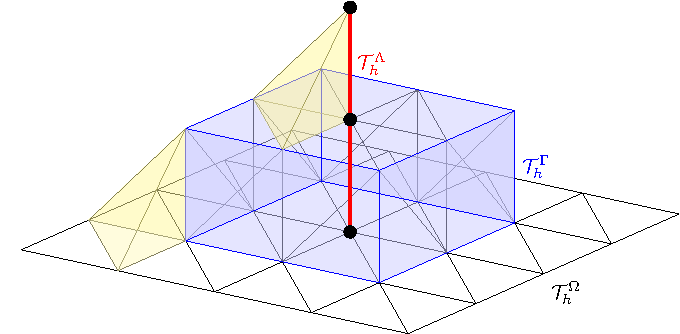
\includegraphics[width=0.5\textwidth]{./conform_mesh.pdf}
    \caption{$\Lambda$ and $\Gamma$ conforming discretization of $\Omega$
      used for \eqref{eq:problem1_simple}. For \eqref{eq:problem2_simple}
      only conformity to $\Lambda$ is needed.
    }
    \label{fig:mesh}
  \end{center}
\end{figure}
  
Formulations \eqref{eq:problem1_simple} and \eqref{eq:problem2_simple} shall
be discretized using contiuous Lagrange element of order 1 ($P_1$) for all the spaces
involved. We recall that since are are investigating the conforming case, the tripplet
$P_1$-$P_1$-$P_1$ satisfies
the discrete inf-sup condition. The resulting linear systems are solved
using the minimal residual method (MinRes) with stopping criterion requiring the relative
preconditioned residual norm to be less than $10^{-12}$. As the preconditioner
we use the (approximate) Riesz mapping with respect to the inner products of
the spaces in which the two formulations were proved to be well posed.
In particular, the preconditioner for the Lagrange multiplier relies on
(the inverse of) the fractional Laplacian $-\Delta^{-1/2}$ on $\Gamma$ for
\eqref{eq:problem1_simple} and $\Lambda$ for \eqref{eq:problem2_simple}.
We remark that the size of the linear systems on the finest meshes considered
here prevents the use direct solvers. Therefore iterative solvers were necessary. 

Considering uniform refinements of the initial mesh, Table \ref{tab:error_conform}
lists the errors of formulations \eqref{eq:problem1_simple} and \eqref{eq:problem2_simple}
on the benchmark problem. It can be seen the error in $u$ and $\ud$ in $H^1$ norm
converges linearly (as can be expected due to $P_1$ element discretization).
Moreover, the error of the Lagrange multiplier approximation in $H^{-1/2}$ norm
decreases quadratically. In the light of $P_1$ discretization this rate appears
superconvergent. We speculate that the result is due to the fact that the
exact solution is particularly simple, $L=0$. In case of the results for
\eqref{eq:problem1_simple} the rate can also be due to the fact that the
error is interpolated into the same finite element space as the approximation $L_h$.
We remark that for $u$ and $\ud$ the error is interpolated into FE space of piecewise
quadratic \emph{discontinous} functions. For \eqref{eq:problem2_simple} we
evaluate the fractional norm and interpolate the error using piecewise continuous
cubic functions. Evaluating the fractional norm in higher order spaces
for formulation with the multiplier space on $\Gamma$ is prohibitively costly. 

%
\begin{table}
  \scriptsize{
    \begin{minipage}{0.49\textwidth}
  \begin{center}
    \begin{tabular}{c|ccc}
      \hline
    $h$ & $\norm{u-u_h}_{1, \Omega}$ & $\norm{\ud-\udh}_{1, \Lambda}$ & $\norm{L-L_h}_{-1/2,\Gamma}$\\
      \hline
4.3E-1 & 3.4E0(--) & 5.3E-1(--) & 2.9E0(--)\\
2.2E-1 & 1.7E0(0.99) & 2.6E-1(1.06) & 6.1E-1(2.25)\\
1.1E-1 & 8.7E-1(0.99) & 1.3E-1(1.02) & 1.4E-1(2.13)\\
5.4E-2 & 4.4E-1(1.00) & 6.3E-2(1.00) & 3.4E-2(2.03)\\
2.7E-2 & 2.2E-1(1.00) & 3.1E-2(1.00) & 8.6E-3(2.00)\\
\hline
  \end{tabular}
  \end{center}
  \end{minipage}
    }
    \vspace{5pt}
  \scriptsize{%(ii)
    \begin{minipage}{0.49\textwidth}
      \begin{center}
        \begin{tabular}{c|ccc}
      \hline
    $h$ & $\norm{u-u_h}_{1, \Omega}$ & $\norm{\ud-\udh}_{1, \Lambda}$ & $\norm{L-L_h}_{-1/2, \Lambda}$\\
      \hline
4.3E-1 & 3.1E0(--)    & 5.4E-1(--)   & 4.4E-2(--)   \\
2.2E-1 & 1.7E0(0.87)  & 2.6E-1(1.06) & 1.1E-2(2.01) \\
1.1E-1 & 8.6E-1(0.96) & 1.3E-1(1.02) & 2.7E-3(2.01) \\
5.4E-2 & 4.4E-1(0.99) & 6.3E-2(1.00) & 6.7E-4(2.01) \\
2.7E-2 & 2.2E-1(1.00) & 3.1E-2(1.00) & 1.7E-4(2.01) \\
1.4E-2 & 1.1E-1(1.00) & 1.6E-2(1.00) & 4.1E-5(2.01) \\
\hline
  \end{tabular}
  \end{center}
  \end{minipage}
  }
  \caption{Error convergence of \eqref{eq:problem1_simple} and \eqref{eq:problem2_simple}
    on a benchmark problem \eqref{benchmark}. Continuous linear Lagrange
    elements are used.
  }
  \label{tab:error_conform}
\end{table}

In Table \ref{tab:error_conform} one can observe that the two formulations
yield practically identical approximations of $u$ and $\ud$. However, the solution
cost of the two approaches differs. In Table \ref{tab:cost} we summarize the
size of the linear systems solved at each level of refinement and the time
for the iterative solver to converge. Let us first note that the proposed
preconditioners seem robust with respect to discretization parameter as
the iteration counts are clearly bounded. We then see that the solution
time for \eqref{eq:problem1_simple} is about 2 times longer compared to
\eqref{eq:problem2_simple}. This is in addition to the higher setup costs
of the preconditioner which in our implementation involve solving an eigenvalue
problem for the fractional Laplacian. Therefore it is advantageous to keep
the multiplier space as small as possible. We remark that the missing
results for \eqref{eq:problem1_simple} in Table \ref{tab:cost} and \ref{tab:error_conform}
are due to the memory limitations which we encounter when solving the eigenvalue problem
for the Laplacian, which for finest mesh involves cca 32 thousand eigenvalues.
%
\begin{table}
  \scriptsize{
  \begin{center}
    \begin{tabular}{c|cc|ccc|ccc}
      \hline
      $h$ & $\dim{V_h}$ & $\dim{V_{\odot, h}}$ & $\dim{Q^{\Gamma}_h}$ & $\#$ & $T\left[s\right]$ & $\dim{Q^{\Lambda}_h}$ & $\#$ & $T\left[s\right]$\\
      \hline
4.33E-01 &125    &5  &40    &27 &0.03  &5  &9  &0.01\\
2.17E-01 &729    &9  &144   &55 &0.10  &9  &19 &0.02\\
1.08E-01 &4913   &17 &544   &62 &0.25  &17 &36 &0.14\\
5.41E-02 &35937  &33 &2112  &64 &1.97  &33 &42 &1.08\\
2.71E-02 &274625 &65 &8320  &64 &18.01 &65 &36 &8.24\\
1.35E-02 &--     &-- &--    &-- &--    &129 &31 &61.37\\
\hline
    \end{tabular}
    \end{center}
    }
  \caption{Cost comparison of the two formulations. Number of MinRes iterations
    is denoted by $\#$. Time till convergence of the iterative solver (excluding the setup) is shown
    as $T$.
  }
\label{tab:cost}
\end{table}

\textbf{Some plots of the solutions}

%\eqref{benchm_sol3d}-\eqref{benchm_sol1d}

%% \begin{remark}
%% Let us notice that the 3D solution \eqref{benchm_sol3d} is such that $\avrc{u}=0$. Therefore in \eqref{benchmark} it is like we are solving two separated problems, one in $\Omega$ and the other on $\Lambda$.
%% \end{remark}
%% \begin{remark}
%% It would be interesting to make a comparison between the solution of the fully coupled 3D-3D problem \eqref{eq:dirneu} (also in the simplified case of type \eqref{eq:dirneu_simple}) and the solution of the reduced problems \eqref{eq:problem1} and \eqref{eq:problem2}. 
%% Therefore, we could set the values of the data of the problem such that the reduced formulation becomes non-trivial and fully coupled.
%% Then, we will solve both the original and reduced problem to observe the differences in the solutions and the values of the Lagrange multiplier.
%% \end{remark}

\section{Unfitted P1-P1-P0 case}
\subsection{Problem 1} All the observations and the proofs are an application of \cite{burman2014} to our case. Let $\mathcal{T}^{\Omega}_h$ and  $\mathcal{T}^{\Lambda}_{h}$ denote a shape-regular triangulation  of $\Omega$ and an admissible partition  of $\Lambda$ respectively. Let us also introduce the set $\mathcal{G}_h$ of elements of $\mathcal{T}^{\Omega}_h$ intersecting the interface $\Gamma$, namely $\mathcal{G}_h=\left\{ K\in \mathcal{T}^{\Omega}_h : \, K\cap \Gamma \neq \emptyset \right\}$. For the discrete solutions $u_h$ and ${\ud}_h$ of the problem in $\Omega$ and on $\Lambda$ we choose the conforming spaces $X_{h,1}^0(\Omega)\subset H^1_0(\Omega)$ and  $X_{h,1}^0(\Lambda)\subset H^1_0(\Lambda)$ respectively. We extend the Lagrange multiplier $\lambda_h$ to the volume elements of $\mathcal{G}_h$ and we define $Q_h=\left\{\lambda_h: \, {\lambda_h}_{|K}\in P^0(K)\,  \forall K\in \mathcal{G}_h\right\}$. With this choice of the LM space, the problem is not inf-sup stable. We add a stabilization term $-s(\lambda_h, \mu_h)$ and we have
\begin{multline*}
a([u_h, {\ud}_h], [v_h, {\vd}_h]) + b([v_h, {\vd}_h], \lambda_h) + b([u_h, {\ud}_h], \mu_h) - s(\lambda_h, \mu_h)= (f, [v_h, {\vd}_h])\\
 \forall [v_h, {\vd}_h]\in X_h(\Omega)\times X_h(\Lambda) ,\, \forall \mu_h \in Q_h.
\end{multline*}
The stabilization $s(\lambda_h, \mu_h)$ is connected to a projector $\pi_L$ between $Q_h$ and a new space $L_h$ for the LM for which we can prove the inf-sup stability.\\
Therefore we have to build this new space $L_h$, prove that the inf-sup condition is fulfilled, build a projection operator $\pi_L: Q_h \rightarrow L_h$, build $s(\lambda_h, \mu_h)$ and prove that $\forall [u_h, {\ud}_h]$, there exists $\xi_h([u_h, {\ud}_h]) \in Q_h$ s.t.  
\begin{equation}\label{stab_coercivity}
a([u_h, {\ud}_h],[u_h, {\ud}_h] ) + b([u_h, {\ud}_h], \xi_h([u_h, {\ud}_h])) \geq \alpha_\xi \vertiii{[u_h, {\ud}_h]}_{X_h(\Omega)\times X_h(\Lambda) },
\end{equation}
\begin{equation}\label{stab_stability}
(s(\xi_{h}, \xi_{h}))^{\frac 12} \leq c_s \vertiii{[u_h, {\ud}_h]}_{X_h(\Omega)\times X_h(\Lambda) },
\end{equation}
being $\vertiii{\cdot }_{X_h(\Omega)\times X_h(\Lambda) }$ a suitable discrete norm. \\
The space $L_h$ is built as the space of $P^0$ functions defined on macro patches $\left\{ F_j \right\}_j$ of elements of $\mathcal{G}_h$. These patches are such that $diam(F_j)\leq H$ and  $jH\leq |F_j\cap \Gamma|\leq H+h$. Moreover, there exist constants $c_h$ and $c_H$ such that $c_hh\leq H \leq c_H^{-1}h$. To each patch $F_j$ we associate two shape regular macro elements $\omega_j$ and $\tilde{\omega}_j$: $\omega_j$ is built adding to $F_j \cap \Omega_{\oplus}$ a sufficient number of elements of $\mathcal{T}_h^{\Omega}$ contained in $\Omega_{\oplus}$, whereas $\tilde{\omega}_j$ is obtained adding to $F_j \cap\Sigma$ a sufficient number of elements of $\mathcal{T}_h^{\Omega}$ contained in $\Sigma$. Thanks to the shape regularity of these macro elements, we have that the following trace and Poincarè inequalites hold. For every function $v\in H^1(\omega_j)$,
\begin{equation}\label{discr_trace_ineq}
\|Tv\|_{\Gamma\cap \omega_j} \lesssim H^{-\frac 12} \|v\|_{L^2(\omega_j)}
\end{equation}
\begin{equation}\label{disc_poincare_ineq}
\|v- \pi_Lv\|_{L^2(\omega_j)} \leq c_P H \|\nabla v\|_{L^2(\omega_j)},
\end{equation}
being $\pi_L$ the projection onto piecewise constant functions on $F_j$.
The same also in $\tilde{\omega _j}$ for $v\in H^1(\tilde{\omega _j})$. This choice leads to the following stabilization 
\begin{equation*}
s(\lambda_h, \mu_h)= \sum _{K\in \mathcal{G}_h} \int_{\partial K \setminus \partial \mathcal{G}_h} h \llbracket \lambda_h \rrbracket \llbracket \mu_h \rrbracket,
\end{equation*}
being $\llbracket \lambda_h \rrbracket$ the jump of $\lambda_h$ across the internal faces of $\mathcal{G}_h$.
\subparagraph{Is $L_h$ inf-sup stable with constants independent of the cuts?} We have to prove that $\forall l_h \in L_h$, $\exists \beta >0$ s.t.
\begin{equation*}
\sup_{\substack{v_h \in X_{h,1}^0(\Omega),\\ {\vd}_h \in X_{h,1}^0(\Lambda)}} \frac{b([v_h, {\vd}_h], l_h)}{\vertiii{[v_h, {\vd}_h]}} \geq \beta \|l_h\|_{H^{-\frac 12}(\Gamma)}.
\end{equation*}
As in the continuous case, we can choose ${\vd}_h=0$ and we prove that
\begin{equation*} 
\sup_{v_h \in X_{h,1}^0(\Omega),\\ {\vd}_h \in X_{h,1}^0(\Lambda)} \frac{b([v_h, {\vd}_h], l_h)}{\vertiii{[v_h, {\vd}_h]}} \geq  \sup_{v_h \in X_{h,1}^0(\Omega)} \frac{b(v_h, l_h)}{\|v_h\|_{H^1(\Omega)}} \geq \beta \|l_h\|_{H^{-\frac 12}(\Gamma)}, 
\end{equation*}
where $b(v_h, l_h)=(Tv_h,l_h)_{\Gamma} $ with a little abuse of notation. 
Proving the last inequality it is equivalent to find the Fortin operator $\pi_F: H^1_0(\Omega) \rightarrow X_{h,1}^0(\Omega)$, such that 
\begin{equation*}
b(v-\pi_F v, l_h)=0, \quad \forall v\in H^1_0(\Omega), \, l_h \in L_h
\end{equation*} 
and
\begin{equation*}
\|\pi_F v\|_{H^1(\Omega)}\lesssim \|v\|_{H^1(\Omega)}.
\end{equation*} 
We define
\begin{equation*}
\pi_F v = I_h v + \sum _j \alpha _j \varphi _j \qquad \text{with }\alpha_j =\frac{\int_{F_j \cap \Gamma}T(v-I_hv)}{\int_{F_j \cap \Gamma}T\varphi _j}
\end{equation*}
and $\varphi_j \in X_{h,1}^0(\Omega)$ s.t. supp$(\varphi_j)\subset \bar{\omega}_j$, $\varphi_j =0$ on $\partial \omega _j$ and 
\begin{equation*}
 \int_{F_j\cap \Gamma}T\varphi_j=O(H) \text{ and } \|\nabla \varphi\|_{L^2(\omega _j)}=O(1). 
\end{equation*}
This construction is always possible provided $H$ is sufficiently larger that $h$ (usually $H=3h$).
Then $b(v-\pi_F v, l_h)=0 \, \forall l_h$ follows by construction. Indeed:
\begin{multline*}
b(v-\pi_F v, l_h)= \int_{\Gamma} T(v-\pi_Fv)l_h = \sum _j \int_{F_j\cap \Gamma} \left[ T(v-I_hv)-\sum _i \alpha_i T\varphi _i \right]l_h \\
=(\text{supp} \varphi \subset \omega_j) \sum _j \int{F_j\cap \Gamma} \left[ T(v-I_hv)-\alpha_j T\varphi _j \right]l_h\\
=\sum _j \int_{F_j\cap \Gamma} T(v-I_hv) l_h - \frac{\int_{F_j\cap \Gamma} T(v-I_hv)}{\int_{F_j\cap \Gamma}T\varphi_j} \int_{F_j\cap \Gamma}T\varphi _jl_h\\ 
=(\text{using $l_h$ constant on $F_j\cap \Gamma$})\,0.
\end{multline*}
Concerning the continuity of $\pi_F$, we have
\begin{multline*}
\|\nabla \pi_F v \|_{L^2(\Omega)} \leq \|\nabla I_h v\|_{L^2(\Omega)} + \sum_j|\alpha_j|\|\nabla \varphi _j\|_{L^2(\bar{\omega}_j)}
\\
(\text{stability of }I_h)\lesssim   \|\nabla  v\|_{L^2(\Omega)} + \sum_j|\alpha_j|\|\nabla \varphi _j\|_{L^2(\bar{\omega}_j)}
\\
\left(\text{using }\|\nabla \varphi\|=O(1)\right) \lesssim \|\nabla  v\|_{L^2(\Omega)} + \sum_j \frac{\left|\int_{F_j\cap \Gamma} T(v-I_h v)\right|}{\left|\int_{F_j\cap \Gamma}T\varphi _j\right|}
\\
\left(\text{since }\left|\int_{F_j\cap \Gamma}T\varphi _j\right|=O(H)\right) \lesssim  \|\nabla  v\|_{L^2(\Omega)} + \frac 1H \sum_j \left|\int_{F_j\cap \Gamma} T(v-I_h v)\right| 
\\
(\text{H\"older}) \lesssim  \|\nabla  v\|_{L^2(\Omega)} + \frac 1H \sum_j |F_j\cap \Gamma|^{\frac 12} \left(\int_{F_j\cap \Gamma} (T(v-I_h v))^2\right)^{\frac 12}
\\
(\text{being }|F_j\cap \Gamma| \leq H+h)\lesssim   \|\nabla  v\|_{L^2(\Omega)} + \frac {1}{H^{\frac 12}} \sum_j  \| v-I_h v\|_{F_j\cap \Gamma} 
\\
\left(\text{trace inequality} \right)\lesssim   \|\nabla  v\|_{L^2(\Omega)} + \frac {1}{H} \sum_j  \| v-I_h v\|_{L^2(\omega_j)} \lesssim \|\nabla  v\|_{L^2(\Omega)} + \frac {1}{H}  \| v-I_h v\|_{L^2(\Omega)} 
\\
(\text{approximation properties of }I_h)\lesssim \|\nabla  v\|_{L^2(\Omega)}.
\end{multline*}

\subparagraph{Satisfaction of the assumptions of the 
abstract analysis} 
We have to prove \eqref{stab_coercivity} and \eqref{stab_stability}.
We choose the following discrete norm
\begin{equation*}
\vertiii{[u_h, {\ud}_h]}^2_{X_h(\Omega)\times X_h(\Lambda) }
= \|u_h\|^2_{H^1(\Omega)}+|D|\|{\ud}_h\|^2_{H^1(\Lambda)} + \|u_h - {\ud}_h\|^2_{\frac 12, h, \Gamma},
\end{equation*}
where $\|u_h - {\ud}_h\|^2_{\frac 12, h, \Gamma} = \|h^{\frac 12} (u_h - {\ud}_h)\|^2_{L^2(\Gamma)} $.
Concerning the coercivity property \eqref{stab_coercivity}, we have to show that $\forall [u_h, {\ud}_h]$, there esists $\xi_h$ s.t.
\begin{equation*}
(u_h,u_h)_{H^1(\Omega)}+ |D|({\ud}_h, {\ud}_h)_{H^1(\Lambda)} +  (Tu_h -  \mathcal{U}_E {\ud}_h, \xi_h)_{\Gamma} \geq \alpha_{\xi}(\|u_h\|^2_{H^1(\Omega)}+|D|\|{\ud}_h\|^2_{H^1(\Lambda)}+ \|u_h - {\ud}_h\|^2_{\frac 12, h, \Gamma}).
\end{equation*}
We choose 
\begin{equation*}
{\xi_h}_{|F_j\cap \Gamma}=\delta \frac 1H \pi_L(u_h-{\ud}_h) \qquad \text{with } \pi_L(u_h-{\ud}_h) =\frac{1}{|F_j\cap \Gamma|}\int_{F_j\cap \Gamma} Tu_h-\mathcal{U}_E {\ud}_h.
\end{equation*}
Actually, $\xi_h\in L_h \subset Q_h$. Then,
\begin{multline*}
\left( Tu_h - \mathcal{U}_E{\ud}_h, \xi _h \right)_{\Gamma} 
= \sum_j \int_{F_j\cap \Gamma} ( Tu_h - \mathcal{U}_E{\ud}_h)\xi_h
\\
= \delta \frac{1}{H} \sum_j \int_{F_j\cap \Gamma} ( Tu_h - \mathcal{U}_E{\ud}_h) \pi_L(u_h - {\ud}_h)
\\
=\delta \frac{1}{H} \sum_j \int_{F_j\cap \Gamma}  (\pi_L(u_h - {\ud}_h))^2
\\
=\delta \frac{1}{H} \sum_j \left(\|(\pi_L - \mathcal{I})(u_h-{\ud}_h)\|^2_{L^2(F_j\cap \Gamma)}  + \|u_h-{\ud}_h\|^2_{L^2(F_j\cap \Gamma)} \right)
\\
\geq -\delta \frac 1H \sum_j \|(\pi_L - \mathcal{I})u_h\|^2_{L^2(F_j\cap \Gamma)}
- \delta \frac 1H \sum_j \|(\pi_L - \mathcal{I}){\ud}_h\|^2_{L^2(F_j\cap \Gamma)} 
+ \delta \frac 1H \sum_j \|u_h-{\ud}_h\|^2_{L^2(F_j\cap \Gamma)}
\\
\geq -\delta \sum_j c_P^2 \|\nabla u_h\|^2_{L^2(\omega_j)}
- \delta \sum_j c_P^2 \|\nabla  \mathcal{U}_E u_h\|^2_{L^2(\tilde{\omega}_j)}
+ \delta \frac 1H \sum_j \|u_h-{\ud}_h\|^2_{L^2(F_j\cap \Gamma)}
\\
(\text{since }c_H H \leq h ) \leq -\delta c_P^2 \|\nabla u_h\|^2_{L^2(\Omega)} - \delta c_P^2 |\D|\|\nabla {\ud}_h\|^2_{L^2(\Lambda)} + \delta c_H \|u_h-{\ud}_h\|^2_{\frac 12,h,\Gamma}. 
\end{multline*}
With a little abuse of notation we are denoting with $\mathcal{U}_E$ both the uniform extension to $\Gamma$ and $\tilde{\omega}_j$. Therefore, we obtain
\begin{multline*}
a([u_h, {\ud}_h],[u_h, {\ud}_h] ) + b([u_h, {\ud}_h], \xi_h([u_h, {\ud}_h]))
\geq \\
(1-\delta c_P^2) \|\nabla u_h\|^2_{L^2(\Omega)} + (1- \delta c_P^2) |\D|\|\nabla {\ud}_h\|^2_{L^2(\Lambda)}
+\delta c_H \|u_h-{\ud}_h\|^2_{\frac 12,h,\Gamma}
\end{multline*}
and choosing $\delta=\frac{1}{2c_P^2}$ we obtain the coercivity inequality.\\
Concerning the stability inequality, the proof is analogous to the one in \cite{burman2014}.


%-----------------
\bibliographystyle{siamplain}
\bibliography{3d1d_coupled}
\end{document}
